\documentclass{article}
\usepackage[utf8]{inputenc}
\usepackage[margin=1in]{geometry}
\usepackage{listings}
\usepackage{eurosym}
\usepackage{graphicx}
\usepackage{hyperref}
\hypersetup{
	hyperindex=true
}
\usepackage{listings-rust}
\usepackage[utf8]{inputenc}
\usepackage[english]{babel}
\setlength{\parindent}{4em}
\setlength{\parskip}{1em}
\renewcommand{\baselinestretch}{1.5}
\usepackage{tikz}
\graphicspath{ {img/} }
\usepackage{listings}
\usepackage{float}
\usepackage[backend=bibtex,style=numeric,citestyle=numeric,sorting=none]{biblatex}
\addbibresource{bibliography.bib}
\author{Student Number: 170027195}
\title{Dynamic Session Types}
\begin{document}
	\maketitle
	\pagebreak
	\tableofcontents
	\pagebreak
	\section{Literature Review}
	\subsection{Session Types} \label{session types}
	When systems attempt to communicate over a protocol, the constraints of “acceptable” communication must be defined before and during transmission. The rubric to guarantee that protocol communication has fit within these boundaries, is however, less clear. If errors in transmission are to occur, future communication may become infeasible, and at worst, security issues could be introduced.
	
	Honda derived session types\cite{honda1993types, takeuchi1994interaction, honda1998language} as a strategy to mitigate potential issues that stem from the inability to properly check that an implementation of the protocol correctly matches the standard. In the 1994 paper\cite{takeuchi1994interaction} they describe the need for an ``abstraction methodology''to describe interactions between ``multiple, possibly distributed, parallel	processes'', going on to state ``Such organization in turn may well be based on a type discipline, which ensures well-typed programs to behave in a principled fashion''. At its core, the session types proposal is for a language or method of describing the expected protocol communication, with a mechanism to check protocol implementations against the type definition, ensuring their correctness. 	Session types take influence from $\pi$-calculus\cite{milner1999communicating}, a process calculus used to model concurrent systems, with the 1994 paper\cite{takeuchi1994interaction} showing the authors adaption of $\pi$-calculus model of ``synchronous communication of values''.
	
	After the protocol representation has been described, often using the Scribble formal description language\cite{honda2011scribbling}, a checking process can occur to ensure that the implementation of the protocol matches its structure. The checking process can occur using one of three mechanisms, either statically, where the validity of the implementation is checked at compile time, dynamically at run time, or a hybrid approach is used, a combination of compile time assurance with a layer of run time checking also enforced. Such a hybrid approach is described in Hu and Roshida, 2016\cite{hu2016hybrid} a static checker is used to validate the ``behavioural'' aspects of the system, generating finite state machines and restricting operations that can be performed adhere to a defined state. They then describe a ``light'' dynamically checked solution to ensure that defined channels of communication are used, and then are not re-used without throwing an error.
	
	Modern research on session types considers ``multiparty'' systems, while early research largely considered a protocol implementation that exhibited communications between two parties, multiparty communication can have any numbers of participants in protocol communication. A 2008 paper by Honda et al.\cite{honda2008multiparty} gives an example of protocol communication which is extremely difficult to represent in a binary session, giving need for a solution which considers multiparty  communication. The consideration is for a system in which users can purchase expensive books from a seller, two buyers wish to purchase a single book together, the first buyer sends a book title to the seller, who responds to both the first and second buyer with the quote for the price of the book, the first buyer then communicates to the second buyer how much of the price they will pay, the second buyer then finally accepts the quote if they wish to proceed. The authors describe this as ``extremely awkward (if logically possible) to decompose this scenario into three binary sessions'' and express the need for the ability to express this as a single session, validated against a protocol implementation. The paper provides an expansion of the initial session types language found in\cite{honda1998language, takeuchi1994interaction} which incorporates the ability to consider protocols which express the communication between multiple parties over a protocol.
	\subsubsection{Static Session Type Implementations}
	Static implementations of session types, as expressed in section \ref{session types} perform the checking of the validity of the protocol implementation at compile time. There are multiple real world implementations for a host of languages that implement such a system in varying forms, from Java through to Haskell\cite{lindley2016embedding}. 
	
	Some statically typed implementations, such as SessionJ\cite{hu2008session} for Java, implement extensions to the language they are built for to provide this functionality. SessionJ implements a \texttt{protocol} keyword and subsequent domain specific language for expressing the contents of a protocol specification, an example of this is show in listing \ref{lst:sessionJ}. The communication of the structure of a protocol may not be possible, or elegant, without creating such an extension, in the Hu et al. paper\cite{hu2008session} an integration of the language extension into the wider Java compilation process is implemented. They describe three layers of compilation and execution, with the first layer being the "SessionJ source code", the Java code with the protocol extensions implemented, this then is translated into Java by the SessionJ compiler, before running on the JVM with SessionJ run time libraries to ensure that the sending an receiving of messages over the protocol is implemented correctly.
	\begin{lstlisting}[language=java, frame=single, numbers=left, caption=An implementation of a protocol to place an order by Hu et al. to showcase the capabilities of SessionJ\cite{hu2008session}, label={lst:sessionJ}]
protocol placeOrder {
	begin. // Commence session.
	![ 	// Can iterate:
		!<String>. 	// send String
		?(Double) 	// receive Double
	]*.
	!{ 	// Select one of:
		ACCEPT: !<Address>.?(Date),
		REJECT:
	}
}

	\end{lstlisting}
	Other approaches to the implementation of statically checked session types within a language do not extend or modify the language to achieve this functionality. One example, for the Rust programming language\cite{jespersen2015session} uses chained type parameters to achieve their goal, they provide an example of the implementation of an ATM shown in listing \ref{lst:rustlang}, which can take withdrawals and deposits. This displays the syntax with which the session type framework is implemented, through the chaining of a number of calls to types, with \texttt{Recv<>} being to receive a value, and \texttt{Send<>} to send a value over the protocol. Any larger implementation that the ATM example would begin to have extremely long and convoluted type definitions to express the structure of the protocol, effectively becoming a domain specific language for the expression of a protocol's operation within another language. Due to these complexities, such an approach, particularly in the case of statically checked session types which has some form of compilation step to check the validity of the implementation at compile time, does not seem to be favoured.
\begin{lstlisting}[language=rust, frame=single, numbers=left, caption=An implementation of an ATM using session types in Rust\cite{jespersen2015session}, label={lst:rustlang}]
	type Atm = Recv<Id, Choose<Rec<AtmInner>,Eps>>;
	type AtmInner = Offer<AtmDeposit, Offer<AtmWithdraw, Quit>>>;
where:
	type Id = String;
	type Quit = Eps;
	type AtmDeposit = Recv<u64, Send<u64,Var<Z>>>;
	type AtmWithdraw = Recv<u64, Choose<Var<Z>,Var<Z>>>;
	\end{lstlisting}
	\subsubsection{Dynamic Session Type Implementations}
	\subsection{The Actor Model}
	The actor model introduces a model for the control of parallel computation to avoid potential errors, such as deadlock or race conditions. The actor model places a number of rules upon what an actor can do, an actor has 3 valid “actions”; to create another actor, to send a message to another actor or to instruct itself on how to deal with the next message it receives.
	
	Each actor is assigned with some concept of an “address”, this provides a mechanism for an actor to communicate with other actors within the system, passing messages between each other as needed. When messages are passed from one actor to another, they are stored in the actors individual task queue; these tasks are then executed one by one, with an actor polling the queue for new tasks after a single unit of work has been completed. Actors also have some form of private state, this allows for an actor to be aware of information relating to the current status of its execution and the execution of tasks prior to the task is is currently executing. Through these three components, the address, the individual task queue and the private state, a sense of the decoupled nature of the actor model can be realised. The goal is to fully abstract and decouple actors from each other, with communication and synchronisation between actors only occurring via the message passing framework.
	
	There are a variety of implementations of the actor model, some research-focused languages are designed entirely entire around the concept, such as Rosette\cite{Tomlinson:1988:ROC:67387.67410}. Other implementations that are more popular amongst the wider general purpose programming community are Erlang’s concurrent and distributed computation utilities, and Akka, which provides an actor model framework for languages that run on the Java Virtual Machine, such as Scala, Java and Kotlin. 
	Erlang is a functional programming language which has built in message passing capabilities for communication between processes. The \texttt{!} operator is used to send a message to the identified process, an example of a program which sends the word “Ping” to an actor, which then returns “Pong” a number of times is listed in the Erlang documentation\cite{ErlangConcDocs} as displayed in listing \ref{lst:erlangDocs}.
	\begin{lstlisting}[label={lst:erlangDocs}, language=erlang, frame=single, numbers=left, caption=Ping Pong in concurrent Erlang\cite{ErlangConcDocs}]
-module(tut15).

-export([start/0, ping/2, pong/0]).

ping(0, Pong_PID) ->
	Pong_PID ! finished,
	io:format(``ping finished~n'', []);

ping(N, Pong_PID) ->
	Pong_PID ! {ping, self()},
	receive
		pong ->
			io:format(``Ping received pong~n'', [])
	end,
	ping(N - 1, Pong_PID).

pong() ->
	receive
		finished ->
			io:format(``Pong finished~n'', []);
		{ping, Ping_PID} ->
			io:format(``Pong received ping~n'', []),
			Ping_PID ! pong,
			pong()
	end.

start() ->
	Pong_PID = spawn(tut15, pong, []),
	spawn(tut15, ping, [3, Pong_PID]).
	\end{lstlisting}
	Akka's implementation of the actor model provides a similar construct, actors exist within a wider network and pass messages to each other to execution methods. However, unlike Erlang, it provides this as library functionality on top of other general purpose programming languages that run on the Java Virtual Machine. Akka allows developers to create a tree hierarchy of actors, with individual actors organised into groups, as shown in figure \ref{fig:AkkaTree}. This hierarchy is used to enforce concurrency amongst and between groups, with actors inside a group running concurrently as well as the groups themselves. The hierarchical structure of the actor grouping also helps to isolate errors, if a failure of an actor occurs within a group, due to the isolated nature of the actor model this can be dealt with at the group level without requiring a full system-wide recovery process.
	\begin{figure}[H] \label{fig:AkkaTree}
	\caption{Akka actor structure example}
	\centering
	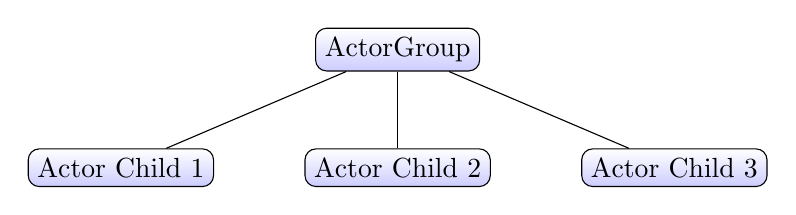
\begin{tikzpicture}[sibling distance=10em,
every node/.style = {shape=rectangle, rounded corners,
	draw, align=center,
	top color=white, bottom color=blue!20}]
\node {ActorGroup}
child { node {Actor Child 1} }
child { node {Actor Child 2} }
child { node {Actor Child 3} };
\end{tikzpicture}
	\end{figure}
	\subsection{Security Problems Regarding Protocols}
	\pagebreak
	\printbibliography
\end{document}